%%%%%%%%%%%%%%%%%%%% author.tex %%%%%%%%%%%%%%%%%%%%%%%%%%%%%%%%%%%
%
% sample root file for your "contribution" to a contributed volume
%
% Use this file as a template for your own input.
%
%%%%%%%%%%%%%%%% Springer %%%%%%%%%%%%%%%%%%%%%%%%%%%%%%%%%%


% RECOMMENDED %%%%%%%%%%%%%%%%%%%%%%%%%%%%%%%%%%%%%%%%%%%%%%%%%%%
\documentclass[graybox]{svmult}

% choose options for [] as required from the list
% in the Reference Guide
\usepackage{amsmath}
\usepackage{mathptmx}       % selects Times Roman as basic font
\usepackage{helvet}         % selects Helvetica as sans-serif font
\usepackage{courier}        % selects Courier as typewriter font
\usepackage{type1cm}        % activate if the above 3 fonts are
                            % not available on your system
%
\usepackage{makeidx}         % allows index generation
\usepackage{graphicx}        % standard LaTeX graphics tool
                             % when including figure files
\usepackage{multicol}        % used for the two-column index
\usepackage[bottom]{footmisc}% places footnotes at page bottom
\usepackage{graphicx}

% see the list of further useful packages
% in the Reference Guide
\usepackage{amsmath}
\makeindex             % used for the subject index
                       % please use the style svind.ist with
                       % your makeindex program

%%%%%%%%%%%%%%%%%%%%%%%%%%%%%%%%%%%%%%%%%%%%%%%%%%%%%%%%%%%%%%%%%%%%%%%%%%%%%%%%%%%%%%%%%

\begin{document}

\title*{Self Healing Microservices Architecture: A case study in Docker Swarm Cluster}
% Use \titlerunning{Short Title} for an abbreviated version of
% your contribution title if the original one is too long
\author{Basel Magableh and Luca Longo}
% Use \authorrunning{Short Title} for an abbreviated version of
% your contribution title if the original one is too long
\institute{Basel Magableh \at Dublin Institute of Technology, Kevien Street, Dublin, Ireland, \email{basel.magableh@dit.ie}
\and Luca Longo \at Dublin Institute of Technology, Kevien Street, Dublin, Ireland \email{luca.longo@dit.ie}}
%
% Use the package "url.sty" to avoid
% problems with special characters
% used in your e-mail or web address
%
\maketitle

\abstract*{Services running in Microservices cluster could be scaled in/out based on the demand issued by end-users, orchestration algorithm, or load balancer running on the cluster leader. The behaviour of Microservices architecture is continuously changing overtime, which makes it a challenging task to use a statistical model to identify normal and abnormal behaviour of the running services. The performance of the cluster nodes could fluctuate around the demand to accommodate scalability, orchestration and load balancing demands. 
 This requires a model that is able to detect anomalies in real-time and generate a high rate of accuracy in detecting any anomalies and a low rate of false alarms. At the same time, it requires dynamic policy configuration that can be used to adapt the recent changes in the operational environment. This paper focuses on proposing a self-healing Microservices architecture, that is able to continuously monitor the operational environment, detects and observes anomalous behaviour, and provides a reasonable adaptation policy using multidimensional utility-based model. We argue in this paper that such model could offer self-scaling of Microservices architecture and adapt the sudden changes in the operational environment. The self-healing property is achieved by means of parameter tuning and dynamic adjustment of the cluster configuration. We believe integrating utility theory in the dynamic decision-making process improves the effectiveness of the adaptation and reduces the adaptation risk including resources over-provisioning and thrashing. Also, it preserving the cluster state by preventing multiple adaptation to take place at the same time.}

\abstract{Services running in Microservices cluster could be scaled in/out based on the demand issued by end-users, orchestration algorithm, or load balancer running on the cluster leader. The behaviour of Microservices architecture is continuously changing overtime, which makes it a challenging task to use a statistical model to identify normal and abnormal behaviour of the running services. The performance of the cluster nodes could fluctuate around the demand to accommodate scalability, orchestration and load balancing demands. 
 This requires a model that is able to detect anomalies in real-time and generate a high rate of accuracy in detecting any anomalies and a low rate of false alarms. At the same time, it requires dynamic policy configuration that can be used to adapt the recent changes in the operational environment. This paper focuses on proposing a self-healing Microservices architecture, that is able to continuously monitor the operational environment, detects and observes anomalous behaviour, and provides a reasonable adaptation policy using multidimensional utility-based model. We argue in this paper that such model could offer self-scaling of Microservices architecture and adapt the sudden changes in the operational environment. The self-healing property is achieved by means of parameter tuning and dynamic adjustment of the cluster configuration. We believe integrating utility theory in the dynamic decision-making process improves the effectiveness of the adaptation and reduces the adaptation risk including resources over-provisioning and thrashing. Also, it preserving the cluster state by preventing multiple adaptation to take place at the same time.}

\section{Introduction}
\label{sec:1}
A Microservices architecture could be defined in the context of a service-oriented architecture as a composition of tiny fine-grained distributed loosely coupled building blocks of software components \cite{stubbs2015distributed}. Microservices improve software modularity and make the application easy to develop and maintain. However, With the rapid development of cloud infrastructures and virtualisation techniques, a high demand for building Microservices architectures in a complete virtualised environment has emerged. This need was met by introducing containers engine like Docker \footnote{https://www.docker.com} as well as cluster management framework such as Docker swarm \footnote{https://docs.docker.com/engine/swarm/}.  
The performance of Microservices running in cluster mode could fluctuate around the demand to accommodate scalability, orchestration and load balancing offered by the cluster leader \cite{stubbs2015distributed}. In their daily base tasks,  many Dev-Ops face an issue of defining and identifying a threshold which can be used to identify a network, system or user activity as normal behaviour. Another challenge that exist in Microservices clusters is the ability to dynamically scale horizontally, (i.e. adjusting the number of nodes participating in the cluster), or vertically (i.e. adjusting the computational resources available for the services). In addition to this, it is not possible to configure auto scaling policy that could be used by the cluster leader to perform resilient and autonomous reasoning to achieve the desired QoS of the architecture. 

Nowadays, cluster management technology does not embed a component that can guarantees continuous monitoring and adaptation of the operation environment and that can offer the architecture dynamic and self-adaptive capability to perform  changes at run-time. To achieve such a high level of scalability, a swarm cluster, for instance, should have a component for continuously monitoring the cluster and a component for adaptation that can implement a reasonable reaction/scaling policy to accommodate the changes in the operating environment. This presents a challenge to build a self-healing microservices architecture that can dynamically adjust its own behaviour and heal itself against anomalous behaviour detected at real-time. Self-healing refers to a property of a self-adaptive software to have the capability of discovering, diagnosing and reacting to disruptions. It can also anticipate potential problems and, accordingly, take proper actions to prevent a failure \cite{Salehie:2009p3693}. To achieve a high level of  self-healing it is necessary to have four major functionalities at run-time: 1) Monitoring and detecting events (contextual changes), 2) Context reasoning (dynamic decision making), 3) Adaptation strategies, 4) validation and verification of the adaptation action \cite{Kapitsaki:2009p3694}.  

%This research focuses on the proposal of a model that can continuously observe and monitor microservices architectures and can detect anomalous behaviour with high accuracy with a minimal low rate of false alarms. At the same time, this model is envisioned to respond to true positive alarms by suggesting a set of adaptation policies (adaptation strategy) using a multi dimensional utility-based model, which can be used by the architecture to select the best adaptation strategy.

The proposed model in this paper offers Microservices architecture a self-healing property by providing a mechanism for continuous monitoring, context detecting of anomalous behaviour using real-time unsupervised anomaly detection algorithm, dynamic decision making using a multidimensional utility based model, enabling dynamic adaptation horizontally or vertically based on the demand and the changes of the operational environment, and runtime verification and validation of the fitness of proposed adaptation strategy. We argue that the self-healing attribute of Microservices architecture is achieved by leveraging parameter tuning and dynamic decision-making supported by an accurate anomaly detection of Microservices architecture. 

This paper is structured as follows: Section \ref{sec:related-work} provides an overview of self-healing architectures and surveys the approaches for  anomaly detection, and run-time configurations. Section \ref{sec:modelling} presents a model that can continuously observe Microservice architectures with Self-healing capabilities. Section \ref{sec:evaluation} proposes a strategy for analysing and evaluating the capability of the model  to detect anomalous behaviours and to trigger suitable adaptation actions. Section \ref{sec:disc} is focused on results found followed a by a critical discussion of the effectiveness of this model. Section \ref{sec:Conclusion} summarises this research, highlighting its contribution and setting future work.


\section{Design and methodology}
%\section{Self-healing Microservices Architecture}
\label{sec:modelling}
\subsection{Self-healing Microservices Architecture}
One important aspect of a self-healing Microservices architecture is the ability to continuously monitor the operational environment, detect and observe anomalous behaviour, and provide a reasonable policy for self-scaling, self-healing, and self-tuning the computational resources to adapt a sudden changes in its operational environment dynamically at rune-time.  
\begin{figure*}[!ht] 
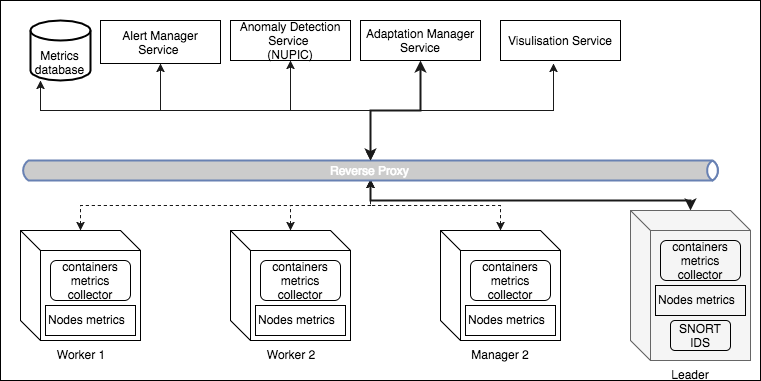
\includegraphics[scale=0.5]{design.png}
\caption{Microservices Architecture implemented in Docker Swarm}
\label{fig_model}
\end{figure*}

To validate the ideas presented in this paper, we design and develop a working prototype of Microservice architecture in Docker swarm \footnote{https://docs.docker.com/engine/swarm/} as shown in Figure \ref{fig_model}. The cluster consisted of many managers and workers. Each cluster has one leader. To meet scalability and availability, the cluster leader distributed the work load between the workers based on Raft Consensus Algorithm \cite{ongaro2015raft}. This means that each service could be executed by assigning multiple containers across the cluster's nodes. 

The main services implemented in this architecture are: Time series metrics database for context collection, Nodes metrics used to collect metrics from all nodes in the cluster, Alert and notification manager used to notify the adaptation manager about contextual changes offered by  Prometheus framework \footnote{https://prometheus.io}. Docker containers metrics collector for collecting fine-grained metrics about all running containers in all nodes \footnote{https://github.com/google/cadvisor}. Reverse proxy for routing traffic between all services in the cluster \footnote{https://caddyserver.com/docs/proxy}. Unsupervised Real-time Anomaly Detection based on NUPIC \footnote{http://nupic.docs.numenta.org/stable/index.html}, Adaptation manager for executing, validating the adaptation actions developed as a prototype of this research. Time series analytic and visualisation dashboard for observing the behaviour of the Microservices cluster \footnote{https://grafana.com}. 
 
This model offering the Microservices architecture with the following functionalities: 

\textbf{Metric collection}: Continuous collection of fine-grained metrics about cluster nodes, services, and containers including (CPU usage, Memory, Disk Reads Bytes/sec, Network Read/s, network write/s and Disk Writes Bytes/sec). The data are streamed into anomaly detection service at real-time. 

\textbf{Model Training}: The NUPIC anomaly detection service \cite{AHMAD2017134} is continuously running over the streamed data collected in Step 1, which enables the generation of the training model for the collected metric.  

\textbf{Anomaly Detection}: The collected real-time data is feed on the fly to NUPIC anomaly detection service \cite{AHMAD2017134}, which provides two features: First, continuous detection of anomalous behaviour with high accuracy. Second, it also provides predictions about the architecture performance based on the collected historic data. This can alerts the architecture about incoming spike on resources demand which can be used by the adaptation manager to schedule a proactive adaptation strategy ahead of time. In addittion, the anomaly detection service is able to detect anomalies as early as possible before the anomalous behaviour is interrupting the functionality of the running services in the cluster as demonstrated by Ahmad et al. \cite{AHMAD2017134}. 

\textbf{Adaptation Election}: Once their is an anomalous behaviour detected with high anomaly score and likelihood, both values are calculated by the Anomaly Detection Service as shown in Figure \ref{fig_model}. The Alert manager notifies the adaptation manager about the anomalous detected. The adaptation manager selects the adaptation action(s) after calculating the utility value for all actions as explained in the following Section \ref{sec:mapk}. Then, the adaptation manager uses the input of the anomaly likelihood, architecture constraints (specified by the DevOp during deployment), and desired/predicted QoS to calculate the best variation of the adaptation that has the highest utility. 


\textbf{Adaptation Execution}: The adaptation manager executes the strategies based on the aggregated value of the utility returned by the algorithm. Once the adaptation action is completed by the adaptation manager, a set of adaptation actions are deployed in the architecture. To avoid, conflicts between multiple adaptation polices, the adapter allow the adaptation actions to be fully completed and verified by the cluster leader according to the consensus performed by RAFT, then it will put a cool off timer before initiating new adaptation actions. This technique is used to avoid resources thrashing and preserving the cluster state for auto-recovery. The adaptation manager sends the cluster leader a set of instructions that might involve tuning of cluster parameters, (horizontal scaling), adding/removing nodes, or vertical scaling of Microservice's containers like scaling a service in/out.  

\textbf{Adaptation Verification}: The cluster leader and all managers in the cluster will vote on the adaptation action based on the consensus algorithm \cite{ongaro2015raft}. The vote results is used to validate and verifies the adaptation action. If the adaptation action won the votes, the adaptation action will be executed by the cluster leader, the adaptation manager records the adaptation attempt as successful. If the adaptation action lost the voting process, then the adaptation manager keeps the current state of the cluster and records the adaptation attempt as failed. In both cases, the adaptation manger records the number of attempts used to complete the adaptation actions.   
 
%The evaluation of this model will come in two folds: First, evaluating the consistent behaviour of the cluster by evaluating the state of the swarm after executing a set of adaptation actions. Second, evaluating the accuracy of the anomaly detection algorithms using confusion matrix \cite{kohavi1998confusion},  as described in the following section. 


\subsection{Adaptation Election}
\label{sec:mapk}
This research focuses on defining a model to continuously observe and monitor the swarm cluster and be able to detect anomalous behaviour with a high accuracy and generate a low rate of false alarms. Then provide the architecture with adaptation strategies with high utility to reason about the detected anomalies and be able to self-adjust the architecture parameters and verifies the adaptation actions at runtime without human intervention.  

For this aim, This research focuses on proposing a model that can continuously observe and monitor the Microservices architecture and be able to detect anomalous behaviour with high accuracy and generate low rate of false alarms. At the same time, the architecture should be able to respond to True positive alarms by suggesting a set of adaptation policies (adaptation strategy), that can be deployed in the cluster to achieve high level of self-healing in response to changes in its operating environment.  

To provide this model with dynamic policy election that guarantees high accuracy of selecting the best adaptation action that fits in the current execution context. The adaptation manager implements a policy election process by employ a utility function to calculate the probability of transition from one state to another. This where the anomaly detection service plays a significant role. At each state $s$ of the Microservice architecture there is a set of context values $c_{1},...,c_{m}$ measuring the matrices of operating environment such as: CPU, Memory, Disk I/O and Network. 

The Anomaly detection service reads the current values of all matrices and calculates the Anomaly Score $as_{1},..., as{m}$ and Anomaly Likelihood $al_{1},...,al_{m}$ of the current metric value in the current state. The anomaly likelihood is accurately defining how anomalous the current metric value comparing to the distribution of learned values by the anomaly detection service. This enables the adaptation manager to scale the weight of each metric value over the distribution value calculated and aggregated in the anomaly likelihood value. The anomaly likelihood is a scaler value between 0 to 1, meaning if the $al_{cpu}$ is 1 and the CPU usage value is 70\% then this might give this metric high utility dimension so it might to be considered in the next adaptation action, so the adaptation manager will select an adaptation policy that can reason about the anomalous behaviour of the CPU value. In another scenario, if the anomaly likelihood is 0, this would give the metric low utility dimension so it will not be considered in the next adaptation action by the adaptation manager as it will return a low reward to the algorithm. 
 
 
\begin{equation}
\label{eq_1}
W(al_{m},C_{m}) =  \max (\sum_{i=1}^{m} al_{i} * c_{i})
 
\end{equation}

 
 
From utility theory, a von Neumann-Morgenstern utility function $U_{i} : X_{i} \rightarrow {R}$ assigns a real number to each quality dimension i, which we can normalize to the range [0, 1] \cite{fishburn1979two}. Across multiple dimensions of contextual changes $C_{m}$, we can attribute a percentage weight to each dimension to account for its relative importance compared to other dimensions. These weights form the utility preferences. The overall utility is then given by the utility preference $w(c_{m})$ function calculated using equ. \ref{eq_1}. For example, if three objectives, u(cpu), u(memory), u(disk), are given anomaly likelihood as follows: the first is twice as important as the second, and the second is three times as important as the third. Then the weight would be quantified as $[w1 : 0.6, w2 : 0.3, w3 : 0.1]$, where the weight is the Anomaly Likelihood of each metric. This gives the CPU metric higher priority to be consider in the adaptation action.
 

In this paper. We argue that the use of anomaly likelihood to weight the collected metrics provides an accurate calculation of the utility function and provides the model with better estimation of the adaptation action. So the maximum metric is selected using the equation described in \ref{eq_1}. In addition to that, an accurate calculation is needed, that calculates the required number of nodes needed to meet the demand of the adaptation action and at the same time maintain the resource provisioning within the allocated budget by the Dev-Ops. The utility cost of provisioning a new node/container in the architecture is calculated based on the equ. \ref{eq_3}, the $Current(c_{m})$ is the current value of the metric value. The $Predicted(c_{m})$ refers to the Predicted value of the utility dimension. The $AnomScore(c_{m})$ is the Anomaly Score of the utility dimension at time $t_{i}$, and $W_{i}$ is the anomaly likelihood value of metric value. The $Predicted(c_{m})$, $AnomScore(c_{m})$, and $W(c_{m})$ are provided by anomaly detection service implemented based on NUPIC. The $UsageTime(u_{i})$ refers to the total number of hours the node is expected to be used per/day, this value is calculated based on the rate of changes calculated based on equ. \ref{eq_4}. The $Cost(instanceType)$ is the cost in \$ for provisioning an instance per/day, normally this is a constant value specified by the cloud infrastructure provider based on the instance type. Finally, the value of $Cost(u_{i})$ is calculated against the constraint of $budget$ as $ Cost(u_{i})  \leq  budget $, The $budget$ is assigned by the Dev-Op to reflect the value of the available budget, so the adaptation manager will not exceed this value at any case. A negative value returned by $Cost(u_{i})$ function means the number of nodes/replicas in the cluster should be reduced by the adaptation action. 


\begin{figure*}[!ht]   
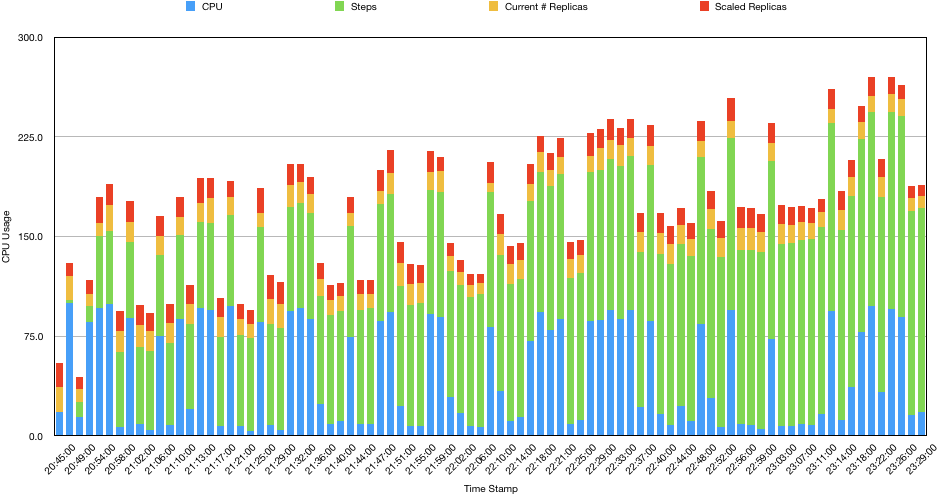
\includegraphics[scale=0.3]{ScalingService.png}
\caption{ Dynamic Scaling of Web Service}
\label{fig_Scale}
\end{figure*} 




\section{Related work}
\label{sec:related-work}
\subsection{Self-adaptive Software}
Self-adaptive software is characterised by a number of properties best referred to as autonomic \cite{jelasityself}. These the `self-* properties' include Self-organisation, Self-healing, Self-optimisation and Self-protection  \cite{horn:2001p3735}. Self-healing architecture refers to  the capability of discovering, diagnosing and reacting to disruptions. It can also anticipate potential problems and, accordingly, take suitable actions to prevent a failure \cite{horn:2001p3735}. Self-healing aspects of Microservices architectures requires a decision-making strategy that can work in real-time. This is essential for Microservice to reason about its own state and its surrounding environment in a closed control loop model and act accordingly \cite{Cheng:2008p3708}.  
Typically, a self-adapting system follows MAPE-K model (Monitor-Analyse-Plan-Execute over a shared Knowledge). a self-healing system should implements MAPE-K model including: Gathering of data related to the surrounding context (Context Sensing); Context observation and detection; Dynamic decision making; Adaptation execution to achieve the adaptation objectives defined as QoS; Verification and validation of the applied adaptation actions in terms of its ability to meet the adaptation objectives and meet the desired QoS.
\subsection{Context Sensing}

 However, there is many approaches are used for achieving high level of self-adaptability though Context sensing involving context collection, observation and detection of contextual changes in the operational environment \cite{Strang:2004p3770}. Also, the ability of the system to dynamically adjust its behaviour can be achieved using parameter-tuning \cite{Cheng:2009p3902}, component-based composition \cite{MariusMikalsen:2005ur}, or Middleware-based  approaches \cite{CheungFooWo:2007p1692}. Another important aspect of self-adaptive system is related to its ability to validate and verify the adaptation action at runtime based on Game theory \cite{Wei:2016ge}, Utility theory as in \cite{Menasce:2007vq,KonstantinosKakousis:2008ub}, or Model driven approach as in \cite{Sama:2008p3765}.

Context information (1) refers to any information that is computationally accessible and upon which behavioural variations depend \cite{Hirschfeld:2008p1620}. Context observation and detection approaches (2) are used to detect abnormal behaviour within the microservices architecture at run-time. Related work in context modelling, context detection and engineering self-adaptive software system are discussed in \cite{Salehie:2009p3693,Cheng:2008p3708,RogeriodeLemos:2011tj,Strang:2004p3770}.  
In dynamic decision making and context reasoning (3), the architecture should be able to monitor and detect normal/abnormal behaviour by continuously monitoring the contextual information found in the Microservices cluster. 

\subsection{Adaptation Planing and Execution}
In Microservices cluster, the performance of the cluster nodes could fluctuate around the demand to accommodate scalability, orchestration and load balancing issued by cluster leader. This requires a model that is able to detect anomalies in real-time and generate a high rate of accuracy in detecting any anomalies and a low rate of false alarms. In addition, there will be a set of variations that can be used by the system to adapt the changes in its operational environment. This requires a dynamic decision making that can calculate the utility of all possible adaptation actions based on the architecture constraints (i.e. number of replicas, number of nodes, desired objectives, metrics thresholds), anomaly score of the detected conditions (CPU, Memory, DISK I/O, Network I/O), and the confidence and accuracy of the anomaly score of the detected abnormal behaviour, and the desired/predicted cluster state. Then, the adaptation manager will execute the adaptation action and verifies its successfulness over the cluster architecture. Also, the adaptation manager will be able to self-tune and self-adjust the architecture parameters to meet high/low demand for services. Finally, the architecture will preserve the cluster state through the adaptation cycle (monitoring, observing, detecting, reacting, and verifying). This research focuses on finding a method to continuously observe and monitor the swarm cluster and be able to detect anomalous behaviour with a high accuracy and generate a low rate of false alarms. Then provide the architecture with adaptation strategies with high utility to reason about the detected anomalies and be able to self-adjust the architecture parameters and verifies the adaptation actions at runtime without human intervention.


\subsection{Anomaly Detection}

There are two phases for detecting anomalies in a software system: a training phase which involves profiling the normal behaviour of the system; a second phase aimed at testing the learned profile of the system with new data and employing it to detect normal/abnormal behaviours \cite{Patcha:2007hja}. 

Three major techniques for anomaly detection have emerged from the literature: statistical anomaly detection, data-mining and machine-learning based techniques. 

Within the statistical methods, a system observes the activity of the system and generates profiles of  system metrics to represent its behaviour. The system profile includes performance measures of the system resources such as CPU and Memory. For each measure, a separate profile is stored. Then, the current readings of the system are profiled and compared against the memorised past profile to calculate an anomaly score. This score is calculated by comparing all measures within the profile against a threshold specified by the developer. Once the system detects that the current readings of the system  are higher than this threshold, then these will be automatically categorised as  intrusions thus triggering an alert \cite{kruegel2003anomaly}. 

Various statistical anomaly detection systems have been proposed and they have some advantages \cite{anderson1995next,roesch1999snort}. 
One of this is that they can detect an anomaly without prior knowledge of the system. This can mitigate the common problem of a cold start found in machine learning techniques. Additionally, statistical anomaly detection provides accurate notifications of malicious attacks that occurred over long periods of times and it performs better in detecting denial-of-service attacks \cite{Patcha:2007hja}. 
However, a disadvantage is that a skilled attacker might train a statistical anomaly detection system to accept the abnormal behaviour as normal. It is difficult to determine the thresholds that make a balance between the likelihood of a false negative (the system fails to identify an activity as an abnormal behaviour) and the likelihood of a false positive (false alarms). Statistical methods need an accurate  model with a precise distribution of all measures. In practice, the behaviour of virtual machines/computers cannot be entirely be modelled using solely statistical methods.

With regard to data-mining approaches, data-mining is about finding insights which are statistically reliable, unknown previously, and actionable from data \cite{phua2010comprehensive}. The dataset must be available, relevant, adequate, and clean. The data mining process involves discovering a novel, distinguished and useful data pattern in large datasets to extract hidden relationships and information about the data. In general, there are two issues involved in the use of data mining in an anomaly detection system. First, there is a lack of a large dataset to be used by the algorithm containing lots of information about the architecture. Second, few approaches were targeting the anomaly detection system in Microservices architecture \cite{phua2010comprehensive}. Data mining based anomaly detection systems have three major difficulties which prevent them from being widely adopted in Microservices architecture \cite{Patcha:2007hja}. Firstly, the low accuracy of detecting anomalous behaviour \cite{gupta2016network,Patcha:2007hja}, as the data mining process would require large dataset with longer time interval to be able to improve the accuracy of detection. Most data mining techniques are heavily on computational resources, this negatively influences their adoption in a Microservices architecture \cite{Patcha:2007hja}. Additionally, usually a data mining method used to classify an attack within a specific system cannot be successfully employed within another system for the same purpose. This because the process of training, testing the model and performing classification of anomalies needs to be repeated with different data or architecture \cite{Buczak:2016kt}.  

Machine learning, in the context of  anomaly detection, can allow the creation of  software system able to learn and improve its detection accuracy over time \cite{bujlow2012method}.
Machine learning-based anomaly detection models aims to detect anomalies similar to statistical and data mining approaches. However, unlike them latter which tend to focus on understanding the process that generated the data, the former are data-driven and are mainly focus on training a model based exclusively on past data \cite{Patcha:2007hja}. This means that, when additional and new data is provided they can intrinsically change their detection strategy and classify significant deviations from the normal behaviour of an underlying software program.
An application of Machine Learning which enables the Microservices cluster to distinguish between normal and abnormal behaviour in the data can be found in \cite{Buczak:2016kt}. 
In general, anomaly detection systems uses a combination of clustering and classification algorithms to detect anomalies. The clustering algorithm is used to cluster the dataset and label them. Then, a decision tree algorithm can be used to distinguish between normal and abnormal behaviour.
Golmah \cite{golmah2014efficient} suggested the use of an effective classification model to identify normal and abnormal behaviour in network-based anomaly detection. The usage of Machine Mearning algorithm  in this context can be found in  \cite{golmah2014efficient,haq2015application,Buczak:2016kt}. Due to the  opening deployment and limited resources found in a Microservices cluster, it is very important to use a lightweight approach of data clustering and classification. Due to this issue, this research focuses on proposing an anomaly detection mechanism that is more suitable for the Microservices architecture and can be easily deployed with less footprints on the limited resources found in the tiny containers running in Microservices cluster . 

Numenta Platform for Intelligent Computing (NUPIC) is based on the Hierarchical Temporal Memory (HTM) model proposed in \cite{Hawkins:2007fi}. HTM has been experimentally applied in real-time anomaly detection of streaming data in \cite{DBLP:journals/corr/AhmadP16,DBLP:journals/corr/LavinA15}. The proposed system based on the HTM model claimed to be efficient and tolerant to noisy data. Most importantly it offers continuous monitoring of real-time data and adapts the changes of the data statistics. It also detects very subtle anomalies with a very minimum rate of false positives. In a recent study, Ahmad et al. \cite{AHMAD2017134} proposed an updated version of the anomaly detection algorithm with the introduction of the anomaly likelihood concept. 
The anomaly score calculated by the NUPIC anomaly detection algorithm represents an immediate calculation of the predictability of the current input stream. This approach works very well with predictable scenarios in many practical applications. As there is no noisy and unpredictable data found, the raw anomaly score gives an accurate prediction of false negatives. However, the changes in predictions would lead to revealing anomalies in the system’s behaviour. Instead of using the raw anomaly score, Ahmad et al. \cite{AHMAD2017134} proposed a method for calculating the anomaly likelihood by modelling the distribution of anomaly scores and using the distribution to check the likelihood of the current state of the system to identify anomalous behaviour. The anomaly likelihood refers to a metric which defines how anomalous the current state is based on the prediction history calculated by the HTM model. So, the anomaly likelihood is calculated by maintaining a window of the last raw anomaly scores and then calculating the normal distribution over the last obtained/trained values, then the most recent average of anomalies is calculated using the Gaussian tail probability function (Q-function) \cite{craig1991new}.

\subsection{Reinforcment Learning}
\textit{The goal of reinforcement learning (RL) is to learn a policy that decides sequential actions by maximizing the cumulative future rewards [30]. Recent trends [23, 32, 28, 27] in RL field is to combine the deep neural networks with RL algorithms by representing RL models such as value function or policy. By resorting of the deep features, many difficult problems such as playing Atari games [23] or Go [27] can be successfully solved in semi-supervised setting. Also, several methods were proposed to solve the computer vision problems, such as object localization [3] or action recognition [16], by employing the deep RL algorithms.
There are two popular approaches in deep RL algorithms: Deep Q Networks (DQN) and policy gradient. DQN is a form of Q-learning with function approximation us- ing deep neural networks. The goal of DQN is to learn a state-action value function (Q), which is given by the deep networks, by minimizing temporal-difference errors [23]. Based on the DQN algorithm, various network architectures such as Double DQN [32] and DDQN [37] were proposed to improve performance and keep stability.
Policy gradient methods directly learn the policy by optimizing the deep policy networks with respect to the expected future reward using gradient descent. Williams et al. [38] proposed REINFORCE algorithm simply using the immediate reward to estimate the value of the policy. Silver et al. [28] proposed a deterministic algorithm to improve the performance and effectiveness of the policy gradient in high-dimensional action space. In the work of Silver et al. [27], it is shown that pre-training the policy networks with supervised learning before employing policy gradient can improve the performance. In tracking problem, we train the proposed network with supervised learning to learn the appearance characteristics of the target objects, and train action dynamics of the tracking target with reinforcement learning using policy gradient method.}


\bibliographystyle{spphys}
\bibliography{selfhealingv2.bib} 


%%%%%%%%%%%%%%%%%%%%%%%%% referenc.tex %%%%%%%%%%%%%%%%%%%%%%%%%%%%%%
% sample references
% %
% Use this file as a template for your own input.
%
%%%%%%%%%%%%%%%%%%%%%%%% Springer-Verlag %%%%%%%%%%%%%%%%%%%%%%%%%%
%
% BibTeX users please use
% \bibliographystyle{}
% \bibliography{}
%
\biblstarthook{References may be \textit{cited} in the text either by number (preferred) or by author/year.\footnote{Make sure that all references from the list are cited in the text. Those not cited should be moved to a separate \textit{Further Reading} section or chapter.} The reference list should ideally be \textit{sorted} in alphabetical order -- even if reference numbers are used for the their citation in the text. If there are several works by the same author, the following order should be used: 
\begin{enumerate}
\item all works by the author alone, ordered chronologically by year of publication
\item all works by the author with a coauthor, ordered alphabetically by coauthor
\item all works by the author with several coauthors, ordered chronologically by year of publication.
\end{enumerate}
The \textit{styling} of references\footnote{Always use the standard abbreviation of a journal's name according to the ISSN \textit{List of Title Word Abbreviations}, see \url{http://www.issn.org/en/node/344}} depends on the subject of your book:
\begin{itemize}
\item The \textit{two} recommended styles for references in books on \textit{mathematical, physical, statistical and computer sciences} are depicted in ~\cite{science-contrib, science-online, science-mono, science-journal, science-DOI} and ~\cite{phys-online, phys-mono, phys-journal, phys-DOI, phys-contrib}.
\item Examples of the most commonly used reference style in books on \textit{Psychology, Social Sciences} are~\cite{psysoc-mono, psysoc-online,psysoc-journal, psysoc-contrib, psysoc-DOI}.
\item Examples for references in books on \textit{Humanities, Linguistics, Philosophy} are~\cite{humlinphil-journal, humlinphil-contrib, humlinphil-mono, humlinphil-online, humlinphil-DOI}.
\item Examples of the basic Springer style used in publications on a wide range of subjects such as \textit{Computer Science, Economics, Engineering, Geosciences, Life Sciences, Medicine, Biomedicine} are ~\cite{basic-contrib, basic-online, basic-journal, basic-DOI, basic-mono}. 
\end{itemize}
}

\begin{thebibliography}{99.}%
% and use \bibitem to create references.
%
% Use the following syntax and markup for your references if 
% the subject of your book is from the field 
% "Mathematics, Physics, Statistics, Computer Science"
%
% Contribution 
\bibitem{science-contrib} Broy, M.: Software engineering --- from auxiliary to key technologies. In: Broy, M., Dener, E. (eds.) Software Pioneers, pp. 10-13. Springer, Heidelberg (2002)
%
% Online Document
\bibitem{science-online} Dod, J.: Effective substances. In: The Dictionary of Substances and Their Effects. Royal Society of Chemistry (1999) Available via DIALOG. \\
\url{http://www.rsc.org/dose/title of subordinate document. Cited 15 Jan 1999}
%
% Monograph
\bibitem{science-mono} Geddes, K.O., Czapor, S.R., Labahn, G.: Algorithms for Computer Algebra. Kluwer, Boston (1992) 
%
% Journal article
\bibitem{science-journal} Hamburger, C.: Quasimonotonicity, regularity and duality for nonlinear systems of partial differential equations. Ann. Mat. Pura. Appl. \textbf{169}, 321--354 (1995)
%
% Journal article by DOI
\bibitem{science-DOI} Slifka, M.K., Whitton, J.L.: Clinical implications of dysregulated cytokine production. J. Mol. Med. (2000) doi: 10.1007/s001090000086 
%
\bigskip

% Use the following (APS) syntax and markup for your references if 
% the subject of your book is from the field 
% "Mathematics, Physics, Statistics, Computer Science"
%
% Online Document
\bibitem{phys-online} J. Dod, in \textit{The Dictionary of Substances and Their Effects}, Royal Society of Chemistry. (Available via DIALOG, 1999), 
\url{http://www.rsc.org/dose/title of subordinate document. Cited 15 Jan 1999}
%
% Monograph
\bibitem{phys-mono} H. Ibach, H. L\"uth, \textit{Solid-State Physics}, 2nd edn. (Springer, New York, 1996), pp. 45-56 
%
% Journal article
\bibitem{phys-journal} S. Preuss, A. Demchuk Jr., M. Stuke, Appl. Phys. A \textbf{61}
%
% Journal article by DOI
\bibitem{phys-DOI} M.K. Slifka, J.L. Whitton, J. Mol. Med., doi: 10.1007/s001090000086
%
% Contribution 
\bibitem{phys-contrib} S.E. Smith, in \textit{Neuromuscular Junction}, ed. by E. Zaimis. Handbook of Experimental Pharmacology, vol 42 (Springer, Heidelberg, 1976), p. 593
%
\bigskip
%
% Use the following syntax and markup for your references if 
% the subject of your book is from the field 
% "Psychology, Social Sciences"
%
%
% Monograph
\bibitem{psysoc-mono} Calfee, R.~C., \& Valencia, R.~R. (1991). \textit{APA guide to preparing manuscripts for journal publication.} Washington, DC: American Psychological Association.
%
% Online Document
\bibitem{psysoc-online} Dod, J. (1999). Effective substances. In: The dictionary of substances and their effects. Royal Society of Chemistry. Available via DIALOG. \\
\url{http://www.rsc.org/dose/Effective substances.} Cited 15 Jan 1999.
%
% Journal article
\bibitem{psysoc-journal} Harris, M., Karper, E., Stacks, G., Hoffman, D., DeNiro, R., Cruz, P., et al. (2001). Writing labs and the Hollywood connection. \textit{J Film} Writing, 44(3), 213--245.
%
% Contribution 
\bibitem{psysoc-contrib} O'Neil, J.~M., \& Egan, J. (1992). Men's and women's gender role journeys: Metaphor for healing, transition, and transformation. In B.~R. Wainrig (Ed.), \textit{Gender issues across the life cycle} (pp. 107--123). New York: Springer.
%
% Journal article by DOI
\bibitem{psysoc-DOI}Kreger, M., Brindis, C.D., Manuel, D.M., Sassoubre, L. (2007). Lessons learned in systems change initiatives: benchmarks and indicators. \textit{American Journal of Community Psychology}, doi: 10.1007/s10464-007-9108-14.
%
%
% Use the following syntax and markup for your references if 
% the subject of your book is from the field 
% "Humanities, Linguistics, Philosophy"
%
\bigskip
%
% Journal article
\bibitem{humlinphil-journal} Alber John, Daniel C. O'Connell, and Sabine Kowal. 2002. Personal perspective in TV interviews. \textit{Pragmatics} 12:257--271
%
% Contribution 
\bibitem{humlinphil-contrib} Cameron, Deborah. 1997. Theoretical debates in feminist linguistics: Questions of sex and gender. In \textit{Gender and discourse}, ed. Ruth Wodak, 99--119. London: Sage Publications.
%
% Monograph
\bibitem{humlinphil-mono} Cameron, Deborah. 1985. \textit{Feminism and linguistic theory.} New York: St. Martin's Press.
%
% Online Document
\bibitem{humlinphil-online} Dod, Jake. 1999. Effective substances. In: The dictionary of substances and their effects. Royal Society of Chemistry. Available via DIALOG. \\
http://www.rsc.org/dose/title of subordinate document. Cited 15 Jan 1999
%
% Journal article by DOI
\bibitem{humlinphil-DOI} Suleiman, Camelia, Daniel C. O�Connell, and Sabine Kowal. 2002. `If you and I, if we, in this later day, lose that sacred fire...�': Perspective in political interviews. \textit{Journal of Psycholinguistic Research}. doi: 10.1023/A:1015592129296.
%
%
%
\bigskip
%
%
% Use the following syntax and markup for your references if 
% the subject of your book is from the field 
% "Computer Science, Economics, Engineering, Geosciences, Life Sciences"
%
%
% Contribution 
\bibitem{basic-contrib} Brown B, Aaron M (2001) The politics of nature. In: Smith J (ed) The rise of modern genomics, 3rd edn. Wiley, New York 
%
% Online Document
\bibitem{basic-online} Dod J (1999) Effective Substances. In: The dictionary of substances and their effects. Royal Society of Chemistry. Available via DIALOG. \\
\url{http://www.rsc.org/dose/title of subordinate document. Cited 15 Jan 1999}
%
% Journal article by DOI
\bibitem{basic-DOI} Slifka MK, Whitton JL (2000) Clinical implications of dysregulated cytokine production. J Mol Med, doi: 10.1007/s001090000086
%
% Journal article
\bibitem{basic-journal} Smith J, Jones M Jr, Houghton L et al (1999) Future of health insurance. N Engl J Med 965:325--329
%
% Monograph
\bibitem{basic-mono} South J, Blass B (2001) The future of modern genomics. Blackwell, London 
%
\end{thebibliography}

\end{document}
